\titledquestion{Shortest Path}
\begin{parts}

\part[3] Consider the weighted undirected graph with $4$ vertices, where the weight of edge ${i, j}$ is given by the entry $W_{i,j}$ in the matrix $W$,
\begin{figure}[htbp]
    \centering
    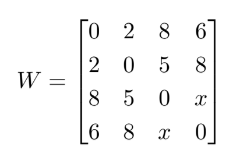
\includegraphics[width=0.2\linewidth]{fig/shortestPath.png}
\end{figure}

We want to find the largest possible integer value of $x$, for which at least one shortest path between some pairs of vertices will definitely contain the edge with weight $x$. What is this largest possible integer value of such $x$? Explain your reason briefly. When breaking tie, the path may be random.

\vspace{1in}



\part[4] Suppose $G = (V, E)$ is a weighted graph and $T$ is its shortest-path from source $s$ to $t$. If we increase all weights in $G$ by the same amount, i.e., $\forall e\in E$, $w'_e=w_e+c$. Is $T$ still the shortest-path from source $s$ to $t$ of the new graph? If yes, prove the statement. Otherwise, give a counter example.
